
\documentclass[withoutpreface,bwprint]{cumcmthesis} %去掉封面与编号页
\usepackage{amsmath}
\usepackage{subeqnarray}
\usepackage{cases}

\usepackage{fontspec}
\usepackage{listings}


    \title{节}
    \begin{document}
        \maketitle
        \begin{abstract}
  


            \keywords{贪心算法\quad  变步长搜索  \quad  坐标变换}
        \end{abstract}


        \section{问题重述}



        \
    
		\subsection{问题1}

        
        
        
        \subsection{问题2}

       
        
        \subsection{问题3} 
       








        \section{问题假设}
        \begin{itemize}
            \item  1:假设天体S离fast射电望远镜足够远,射电望远镜口径与此距离相比可以忽略不计,此时来自天体S的电磁波可视为平行射入。

        \end{itemize}
        

        
        \section{符号假设}

        \begin{longtable}{p{8cm}<{\centering}p{7.5cm}}
            \toprule  %添加表格头部粗线
            符号& 意义\\
            \midrule  %添加表格中横线
            $h$ & 抛物面顶点到基准球面间的距离  \\
            \bottomrule %添加表格底部粗线
        \end{longtable}

        \newpage


        \section{模型建立}

为了预测用户是否遭到的电信诈骗,该问题本质上是一个逻辑回归问题,常用的模型有logistical 回归,
线性回归(Linear Regression), 支持向量机(SVM)等 。
由于单个模型的泛华能力较差,为了获得更高的召回率,准确率,我们这里采用基于
模型融合(Stacking)的方法来求解该逻辑回归的问题。

     所谓模型融合, 在训练数据上训练并使用多个模型进行预测,得到多组预测结果,
     也就是超特征 ,  使用一个新的模型,对这些超特征再进行训练,训练一个从超特征到
     真实值的模型,再将测试数据的超特征输入这些模型,得到最后的结果。   (\ref{fig1a})
     这里我们采用多层模型融合方法,如 (\ref{fig1b})所示的模型融合架构,逐层叠加
     由当个模型加权组合而成的模型来作为最后的模型。

    对于第N层,组合模型,假设对于其中每个模型的输入为:$\vec{Input_{N}}$ ,对应的权重为$W_{Input ,N}$,输出预测结果为$\vec{P_{i,N}}$, 其中i为
    该层的所有模型的编号$\vec{W_{i,N}}$,其对应的权重为。则第N+1层的输入为:
    $ \sum_{\forall i } \vec{P_{i,N}}\bullet \vec{W_{i,N}} +\vec{Input_{N}}W_{Input ,N} $,并且我们
    将数据集分为k块,对不同的模型进行k折交叉验证。通过该操作可以减少方差和降低过拟合。
  
   这里我们使用的多层模型融合具有3层,对于每一层融合模型,其输入为下一层的融合模型输出和单个
   型(这里包括RandomForestGini, WeightedEnsemble\_L2(来自于第二层的融合模型的输出), RandomForestEntr,
   ExtraTreesGini, ExtraTreesEntr, XGBoost, CatBoost,
   NeuralNetTorch, LightGBMLarge, LightGBM, NeuralNetFastAI,
   LightGBMXT, KNeighborsDist, KNeighborsUnif)。
    
     \begin{figure}[H]
        \begin{minipage}[t]{0.5\linewidth}
        
            \centering
            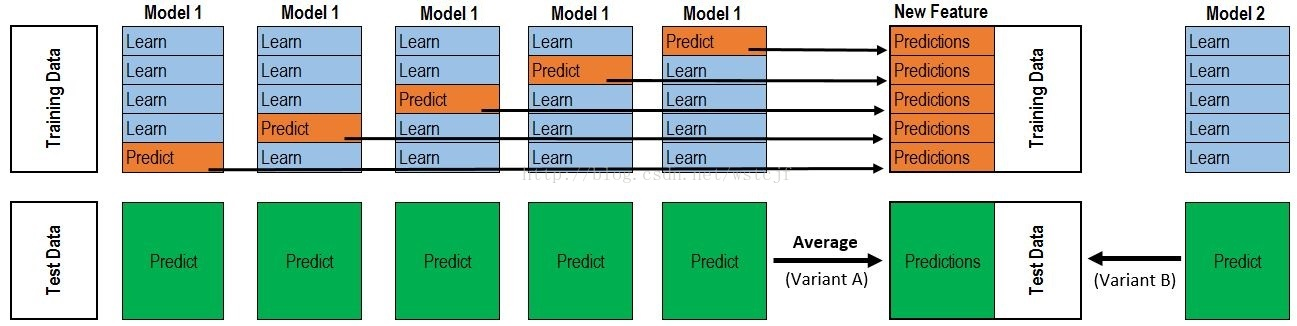
\includegraphics[scale=0.3]{images/moxing.png}
            \caption{模型融合示意图}
            \label{fig1a}
            \end{minipage}%
        \end{figure}

        \begin{figure}[H]
      
                \centering
                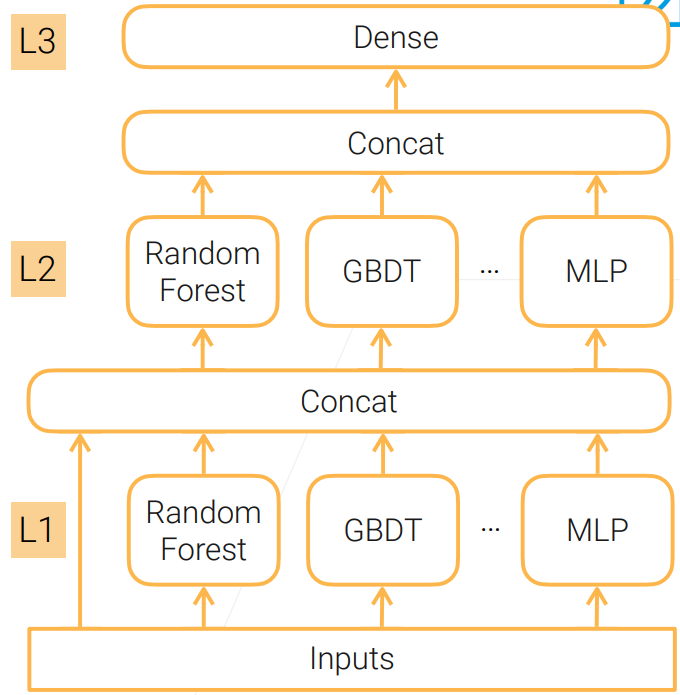
\includegraphics[scale=0.3]{images/stack.png}
                \caption{多层模型融合架构示意图}
                \label{fig1b}

 % 
   
    \end{figure}
        \section{模型求解以及结果分析}


       对于模型的求解,我们使用python进行求解。 
       我们随机选取70\%(70万)的数据用作训练数据,
       将20\%(20万)数据作为测试集,以及将剩下的10\%(10万数据)作为测试集。
       在进行k折交差差验证的训练后,我们的多层融合模型在测试集上取得了
       如下的效果:
       \begin{itemize}
       \item  准确率(accuracy): 0.9999288888888889
       \item   平衡准确率(balanced\_accuracy): 0.9996162978031218 
       \item   马尔萨相关系数(mcc): 0.9995542858142105
       \item   F1分数: 0.9995931703472036
       \item    精度(precision): 0.9999491281842577
       \item   召回率(recall): 0.9992374658448243
       \end{itemize}

       我们分析了该多层融合模型的不同的单个模型在测试集/验证集的得分(\ref{fig2a}),
       从中可与看出,多数模型在验证集以及测试集上的得分(准确率)都是99\% 以上,只有模型
       KNeighborsDist和KNeighborsUnif的得分较低(只有93\%)左右,这可能是因为这两个
       模型都是使用KNN模型进行训练的,是基于每个样本的附近样本来预测该样本,从上文的分析中
       我们知道,由于样本十分不均衡,所以导致了KNN模型得到的结果较差,而在多层融合模型中,
       我们可以通过学习系数权重从而降低KNN模型的影响,所以并不会对结果产生较大影响。
       同时,我们也可以看出,相比于神经网络,随机森林(RandomForestEntr),
       XGBoost等传统模型也可以取得不同的结果,这一点与论文[]的观点一致。
       % Do we need hunrder of t o,,.. 

       
      同时我们也分析了单个模型的在测试集,验证集上的预测耗时(\ref{fig3}),以及训练耗时。
      从中我们可以看到,对于所有模型,在验证集以及测试集上的预测耗时
      极低,基本可以忽略不计,这表明我们选取的模型在训练好进行预测时速度较快。
      但是从训练时间这一项可以看出:对于神经网络类的模型(NeuralNetTorch,
      NeuralNetFastAI),在进行时耗时较长,这也是符合一般经验的,训练神经网络需要
      在每个周期内都进行,梯度下降调参以及损失反向传播,而这两个操作都是比较耗时的。
      而对于传统的机器学习(如随机森林,XGBoost), 其训练时间是可以忽略不计的,
      而且从上文中,我们知道,这种类型的模型也具有较高的精度。但是需要注意的是,
      在参数文件中,神经网络类的模型由于网络参数较多,其参数文件也比较大,大概是
      其他传统机器学习模模型的几个数量级倍。
       
  


       \begin{figure}[H]

        \centering
        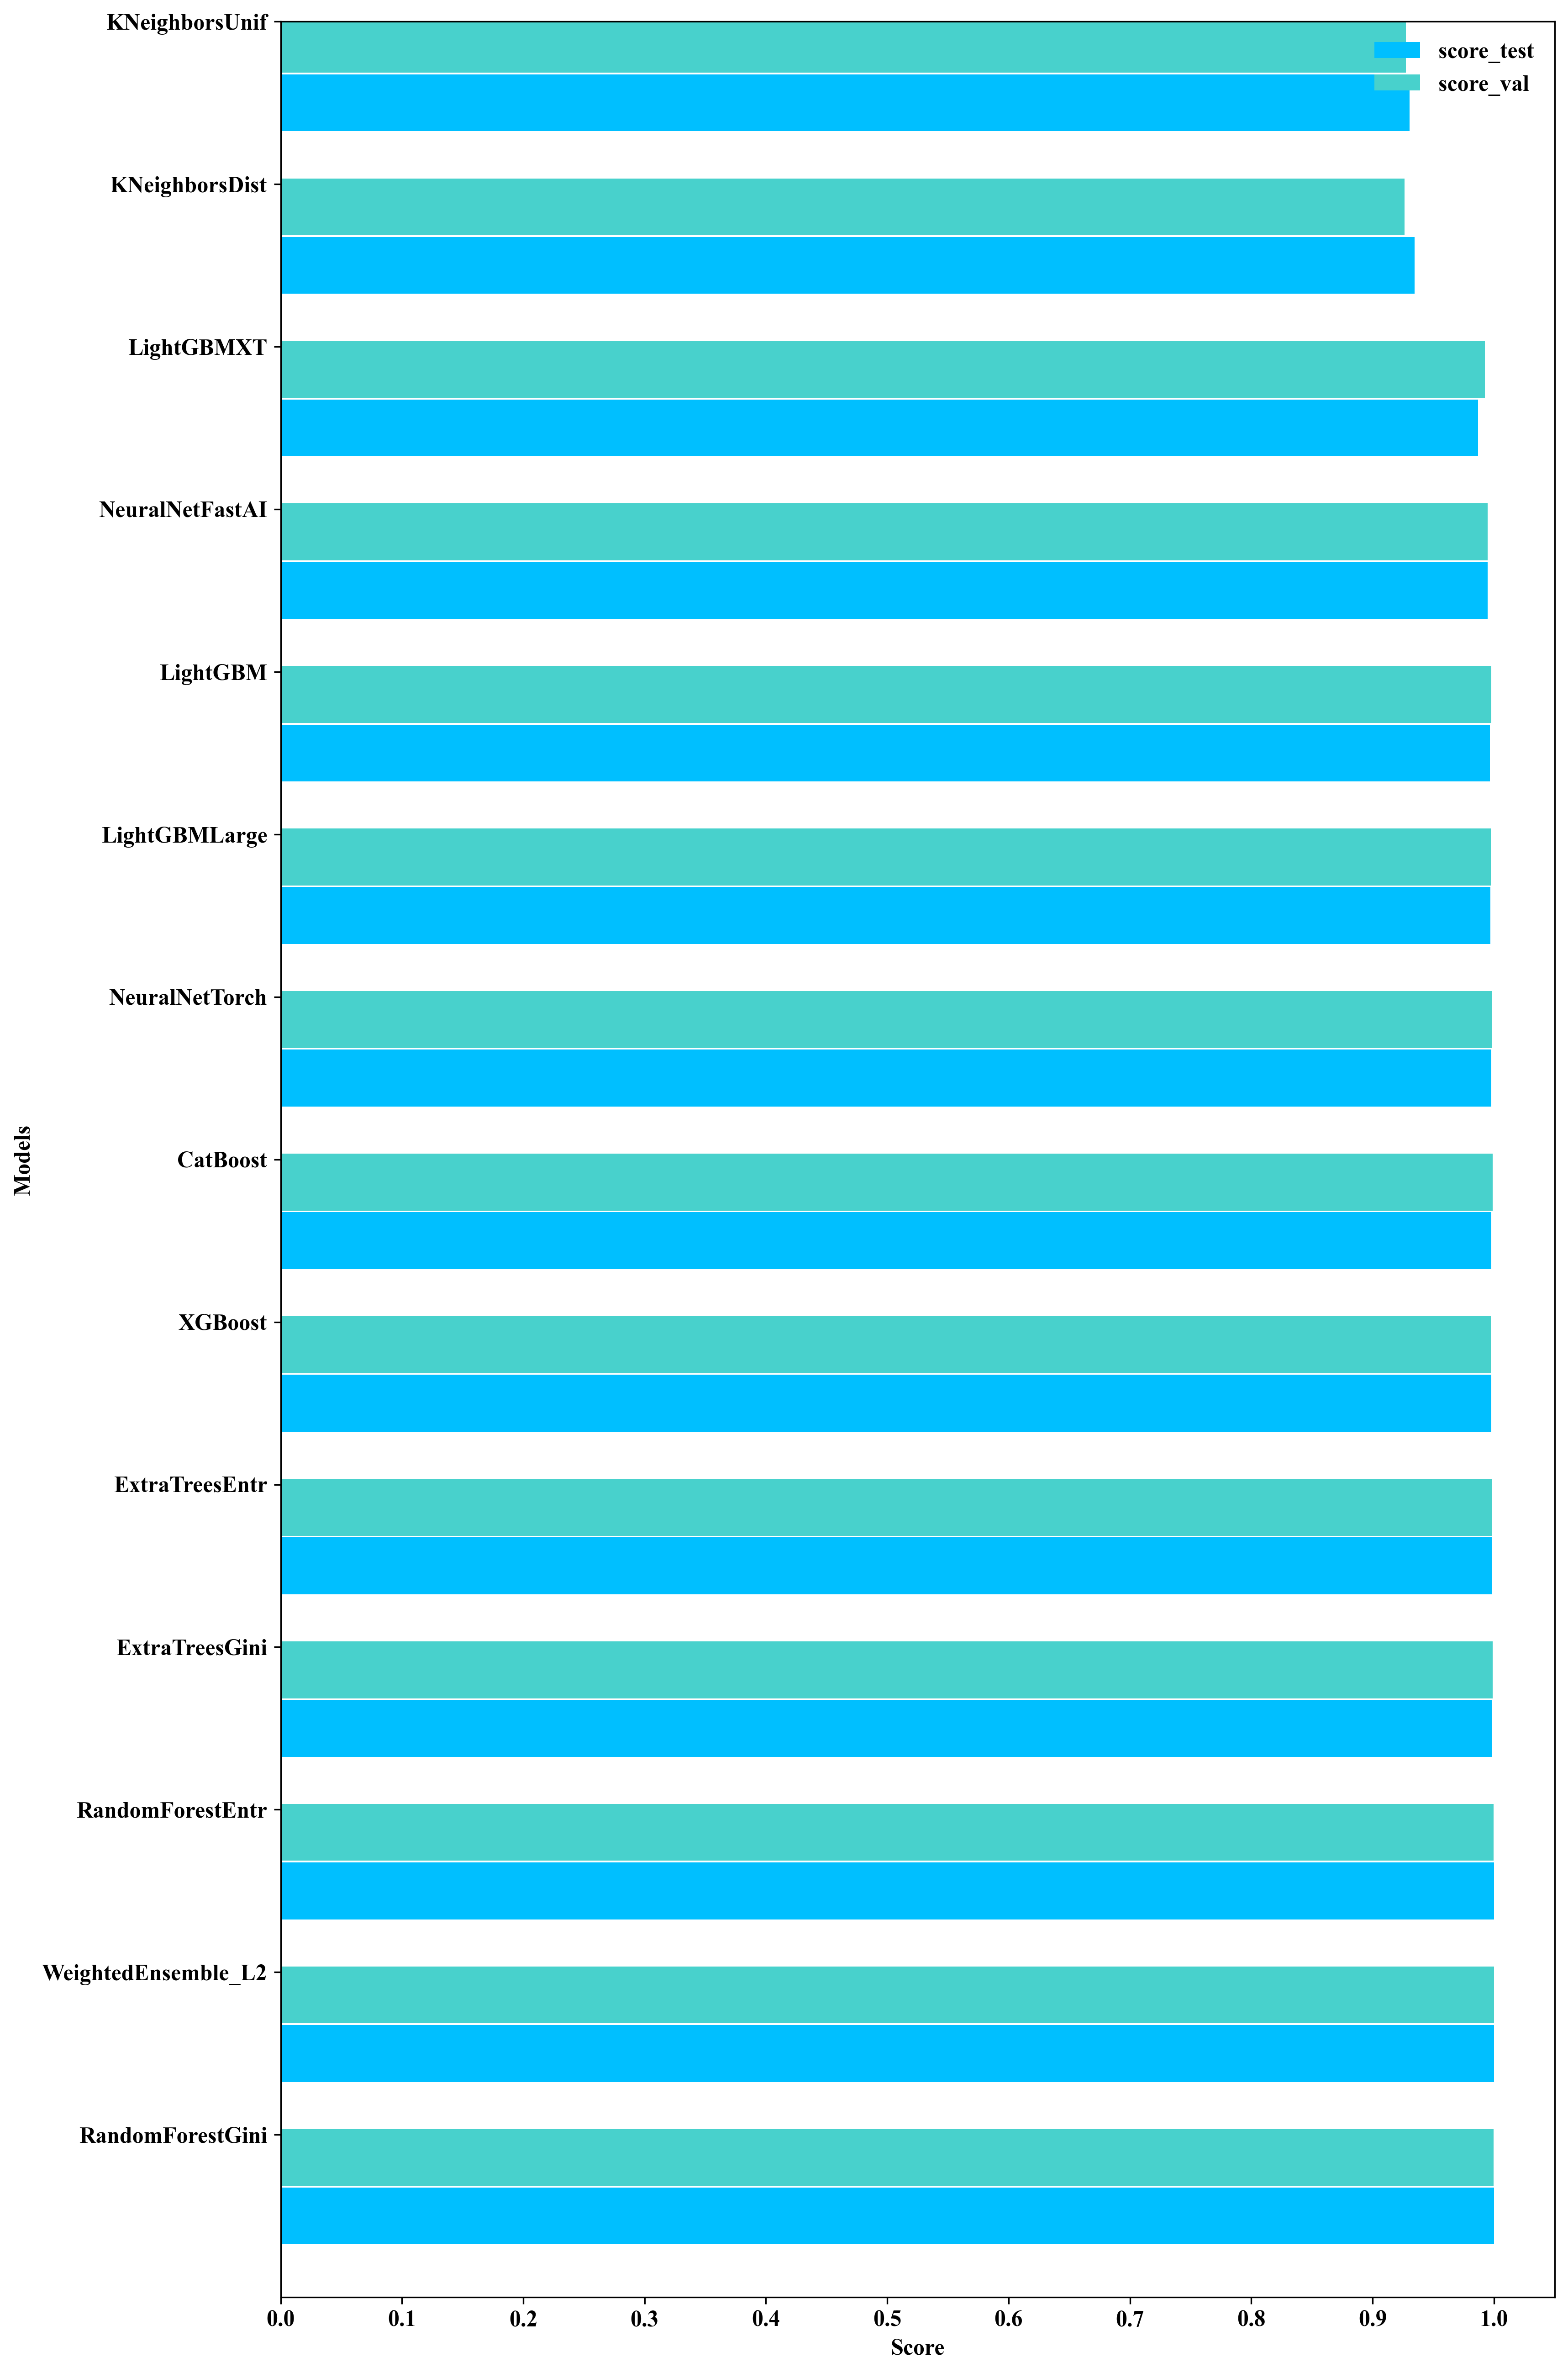
\includegraphics[scale=0.4]{images/score.png}
        \caption{单个模型的验证/测试得分}
        \label{fig2a}


    \end{figure}

    
    \begin{figure}[H]

        \centering
        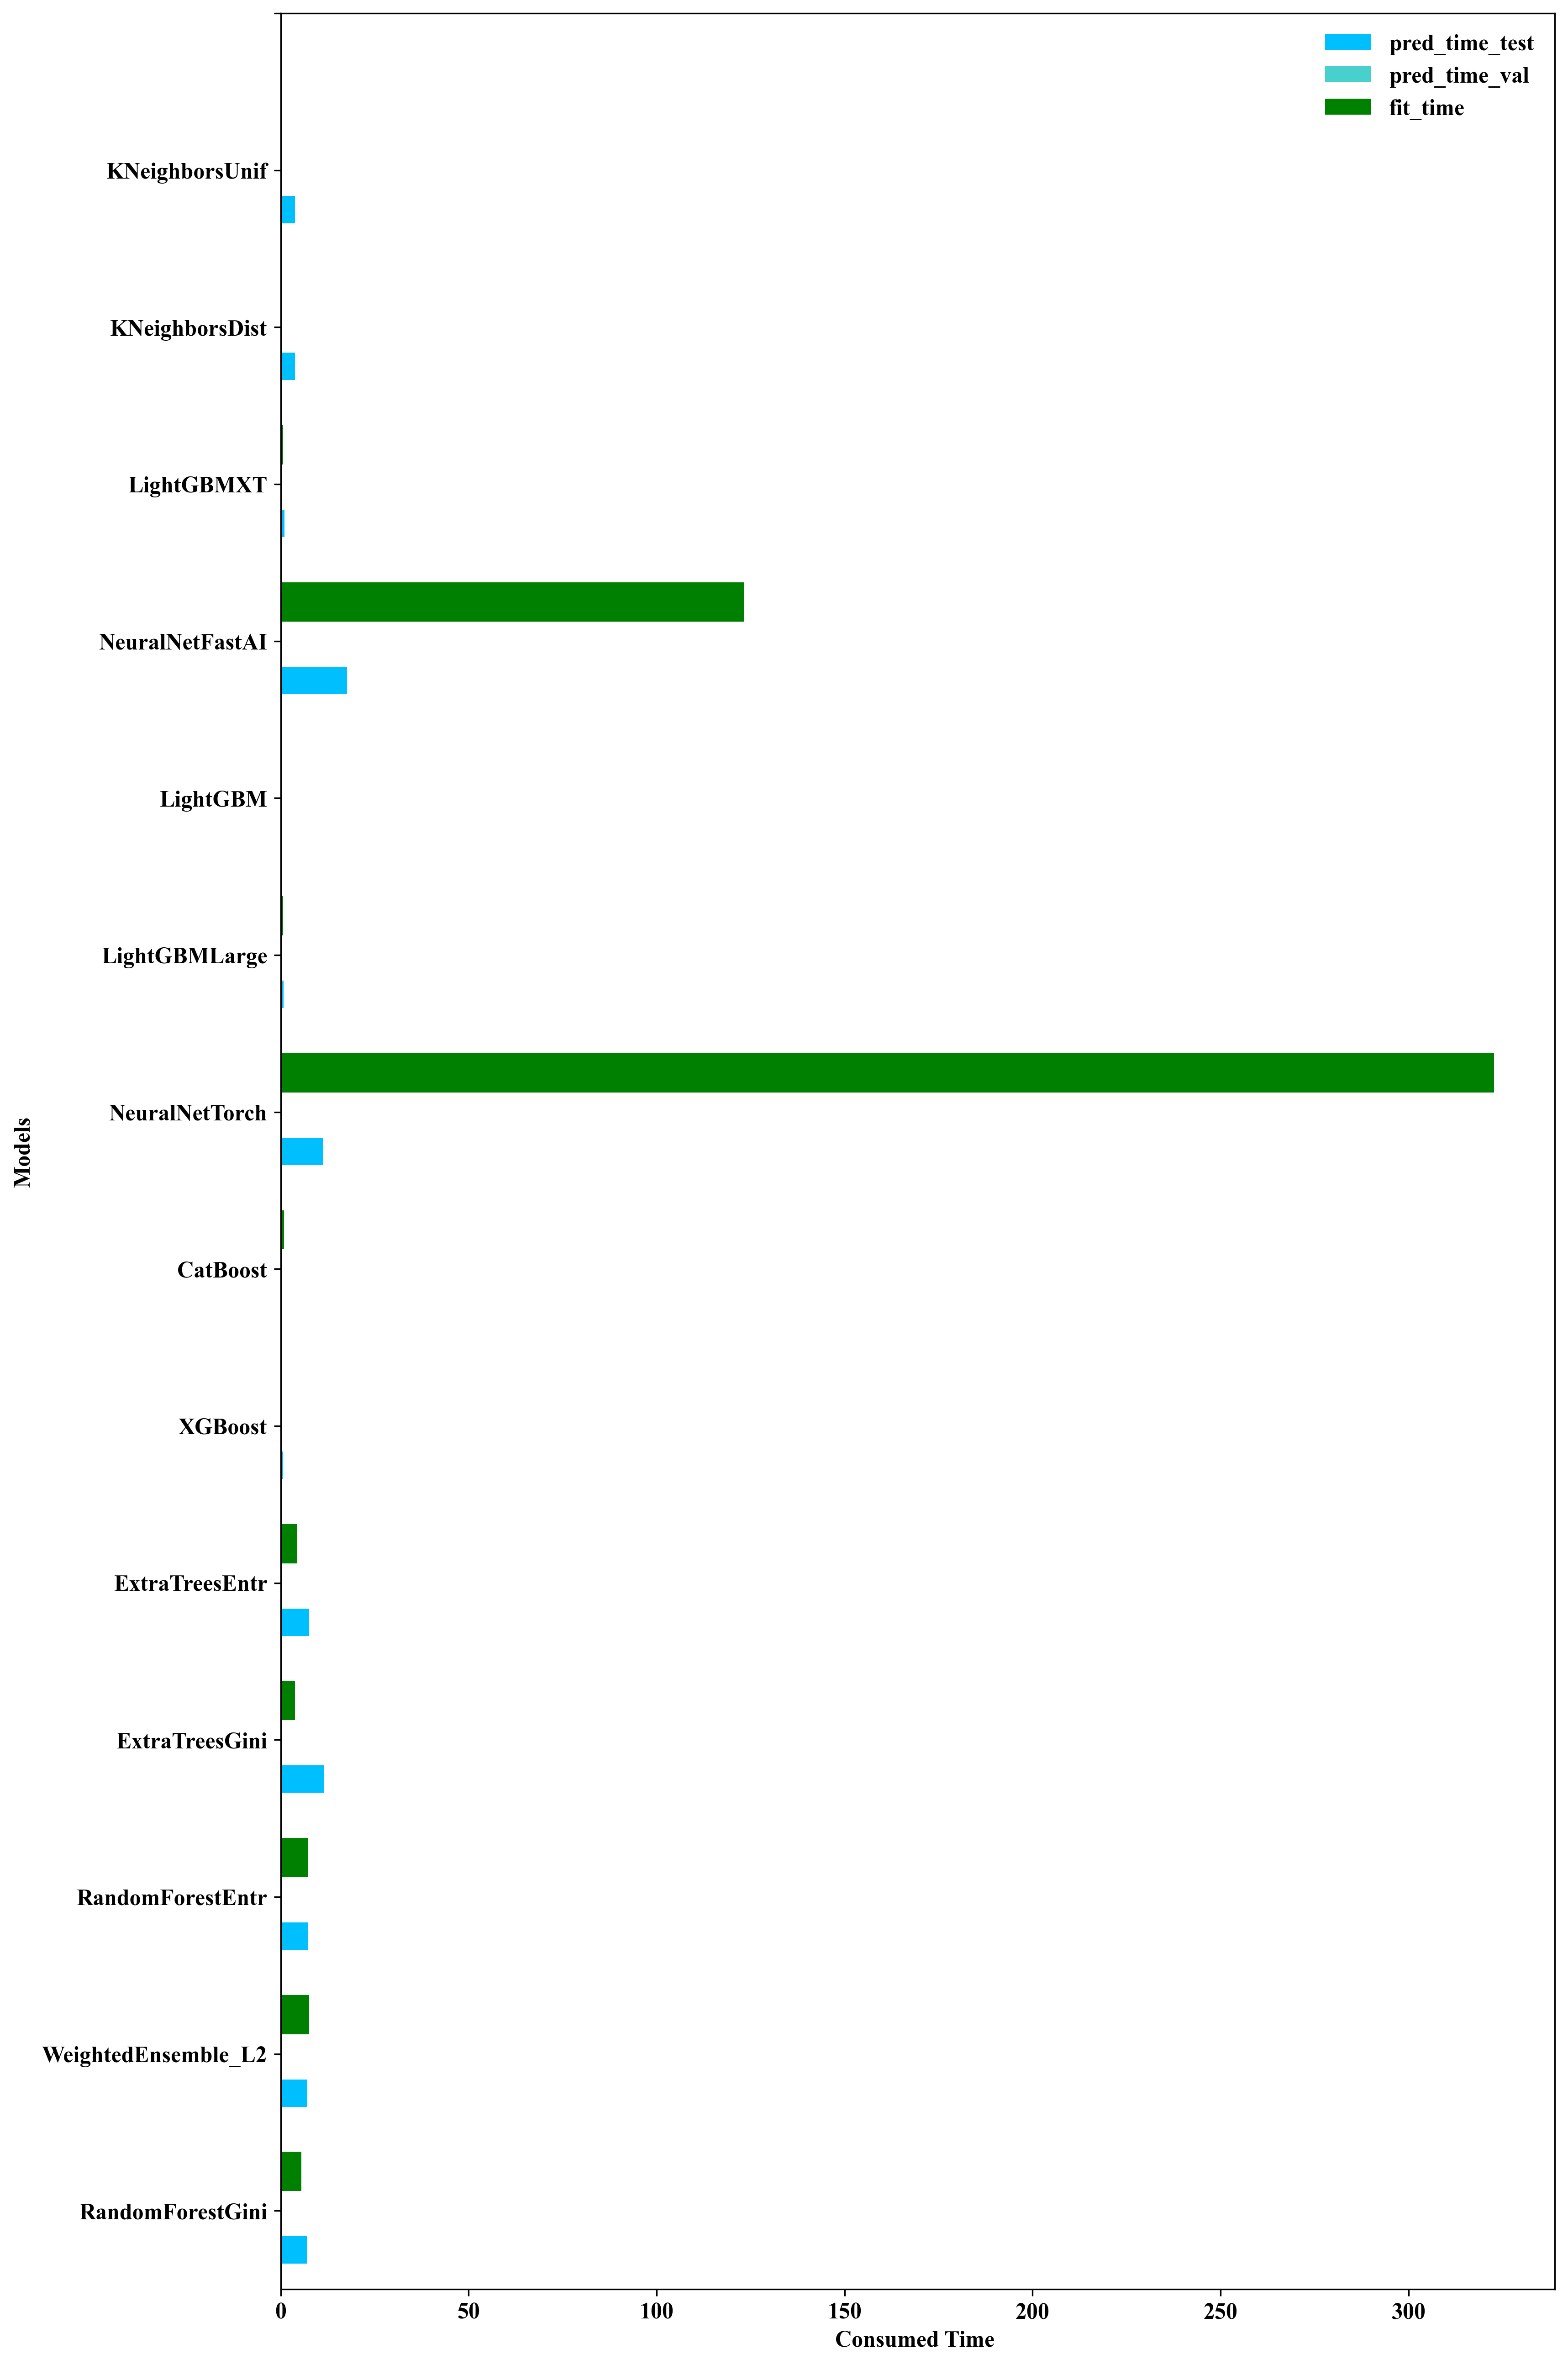
\includegraphics[scale=0.4]{images/times_score.png}
        \caption{单个模型在训练/测试集的预测耗时以及训练耗时}
        \label{fig3}


    \end{figure}

\iffalse 
\begin{figure}[H]
    \begin{minipage}[t]{0.5\linewidth}
    \centering
    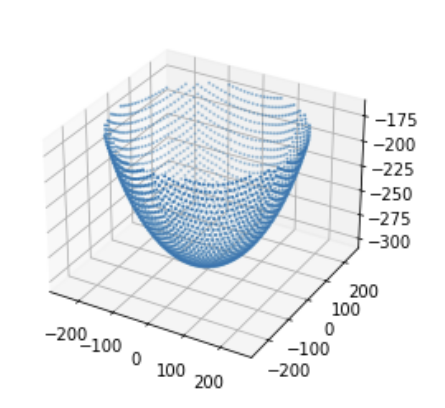
\includegraphics[scale=0.5]{images/allsuo.png}
    \caption{主索节点分布图}
    \label{fig:side:c}
    \end{minipage}%
    \begin{minipage}[t]{0.5\linewidth}
    \centering
    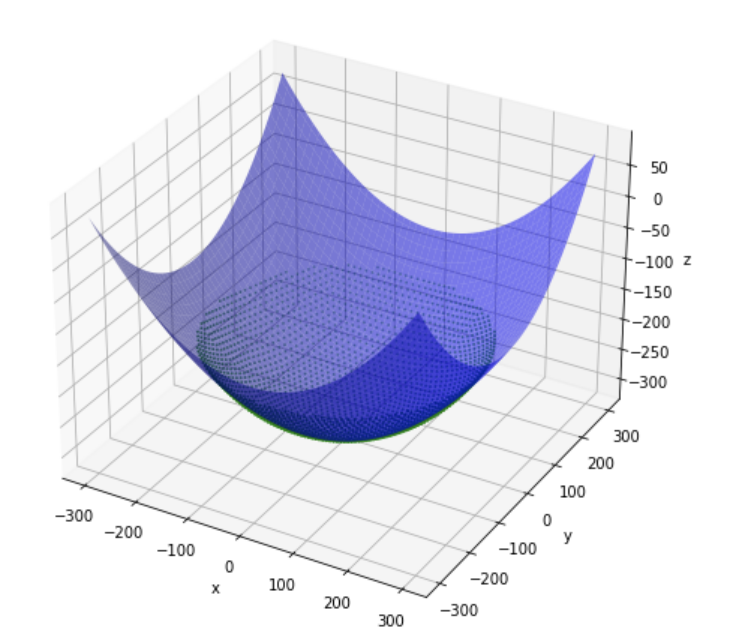
\includegraphics[scale=0.35]{images/zhunbei2.png}
    \caption{300m口径内主索节点分布图}
    \label{fig:side:d}
    \end{minipage}
\end{figure}
\fi 

      



  
\textbf{模型的优化} 




\section{模型的评价与推广}

\subsection{模型的优点}

1.模型参考了"FAST"有关的可靠文献,提出了较合理的衡量反射面板与理想抛物面误差的方案。

2.模型将连续问题离散化,进行变步长搜索,先粗调再细调,搜索速度快,巧妙地解决了优化问题。

3.模型将三维问题转化到二维平面进行分析,进行了相当的简化。

\subsection{模型的缺点}

1.模型近似过程较多,对于光线光路可能存在一定影响。

2.模型所得到的结果难以验证。

3.忽略了馈源舱不同部分接受到的光强差异所产生的影响。

\subsection{模型的改进与推广}

\begin{itemize}
\item 可对于每个反射面板以球面反射进行更细致的分析,进一步提高接受比。
\item 可采用遗传算法等搜索出贪心算法中开始调节的起点。
\item 模型本身在"FAST"球面射电望远镜已经大获成功的前提下具有一定的可行性,
在其他球面结构的望远镜中可同样适用,具有普遍意义。
\end{itemize}



\newpage
    \begin{thebibliography}{9}%宽度9
        \bibitem [1] 
        \newblock 朱丽春.
        \newblock 500米口径球面射电望远镜(FAST)主动反射面整网变形控制[J].
        \newblock 科研信息化技术与应用,2012,3(04):71.

        \bibitem [2] 
        \newblock 李明辉,朱丽春.
        \newblock FAST瞬时抛物面变形策略优化分析[J].
        \newblock 贵州大学学报(自然科学版),2012,29(06):25

        \bibitem [3] 
        \newblock 钱宏亮.
        \newblock FAST主动反射面支承结构理论与试验研究[D].
        \newblock 哈尔滨工业大学,2007:2(27).
       


    \end{thebibliography}


\newpage
    \begin{appendices}

        \section{问题1的代码}
        \begin{lstlisting}[language=python]
          
        \end{lstlisting}

   

    \end{appendices}
\end{document}

